\documentclass{article}
\usepackage{arxiv}

\usepackage[utf8]{inputenc}
\usepackage[english, russian]{babel}
\usepackage[T1]{fontenc}
\usepackage{url}
\usepackage{booktabs}
\usepackage{amsfonts}
\usepackage{nicefrac}
\usepackage{microtype}
\usepackage{lipsum}
\usepackage{graphicx}
\usepackage{natbib}
\usepackage{doi}




\title{Выбор интерпретируемых сверточных моделей глубокого обучения}

\author{ Тимур Мурадов\\
	МФТИ\\
	\And
	Олег Бахтеев \\
	МФТИ\\
	\And
	Константин Яковлев \\
	МФТИ\\
	%% \AND
	%% Coauthor \\
	%% Affiliation \\
	%% Address \\
	%% \texttt{email} \\
	%% \And
	%% Coauthor \\
	%% Affiliation \\
	%% Address \\
	%% \texttt{email} \\
	%% \And
	%% Coauthor \\
	%% Affiliation \\
	%% Address \\
	%% \texttt{email} \\
}
\date{}

\renewcommand{\shorttitle}{\textit{arXiv} Template}

%%% Add PDF metadata to help others organize their library
%%% Once the PDF is generated, you can check the metadata with
%%% $ pdfinfo template.pdf
\hypersetup{
pdftitle={A template for the arrxiv style},
pdfsubject={q-bio.NC, q-bio.QM},
pdfauthor={David S.~Hippocampus, Elias D.~Striatum},
pdfkeywords={First keyword, Second keyword, More},
}

\begin{document}
\maketitle

\begin{abstract}
	В статье рассматривается проблема слабой интерпретируемости сверточных нейронных сетей, то есть затруднённого выделения наиболее важных признаков, а также определения кластеров схожих объектов. Для улучшения интерпретируемоси в статье ведётся модификация доказавшего свою эффективность метода OpenBox работающего с  кусочно-линеными нейронными сетями. Метод обобщается на работу с более широким классом нейронных сетей: сверточными нейронными сетями. Предлагается математически эквивалентная замена слоев: свертка, пулинг, нормализация на линейные, что позволяет значительно улучшить интепретируемость.
\end{abstract}


\keywords{Machine Learning \and CNN \and OpenBox \and Explicit}

\section{Introduction}
При работе со сверточными нейронными сетями частой проблемой является повышение качества, а также анализ получаемых результатов. В данном исследовании стоит задача улучшения интерпретируемости модели, где под интерпретируемостью понимается простота выделения важных признаков на выборке данных и способность относить схожие объекты выборки к одним и тем же кластерам.

Проблемой является в целом высокая сложность интерпретации сверточных нейронных сетей, требующая комплексного подхода. На данный момент существует множество различных решений проблемы интерпретации. В статье [cite{ribeiro2016why}]описан метод \textbf{LIME}, предлагащий линейную апроксимацию предсказаний модели в некоторой небольшой окрестности вокруг объектов из тестовой выборки. Такой подход позволяет получить простую для интерпретации модель, являясь при этом "model-agnostic", то есть никак не использующий информацию о строении модели изнутри, однако он весьма неустойчив к выбросам и сильно зависим от адекватности апроксимации. В статье \cite{Lundberg2017aunified} предлагается другой подход \textbf{SHAP}, заключающийся в рассмотрении вклада каждого признака в результат работы модели, таким образом удается выделять даже скрытые, но значимые признаки, но применимость подхода ограничена ввиду высоких вычислительных затрат, так как требует многократного обучения модели, а также весьма зависим от выборки данных. Ещё один подход к интерпретации \textbf{OpenBox}, описываемый в статье \cite{chu2019exact} редлагает построение математически эквивалентных линейных моделей для линейных нейронных сетей, он показал более высокую эффективность по сравнению с \textbf{LIME} и весьма перспективен для дальнейшей работы.

Задачей проекта является адаптация метода \textbf{OpenBox} для работы со свёрточными нейронными сетями: математически эквивалентно представить в виде линейных моделей такие слои как свёртка, пулинг и нормализация. И доказательство конкурентоспособности по сравнению с другими существующими методами интепретации CNN.

В качестве валидационного датасета предложены: выборка изображений рукописных цифр MNIST и выборка изображений CIFAR-10. Эксперимент выполнялся локально в среде Jupiter Notebook, а также удаленно задействуя графический ускоритель в среде Google Collab. Для построения моделей был выбран язык Python по средствам библиотек с открытым кодом Pytorch и Scikit-Learn.
\bibliographystyle{plain}
\bibliography{Muradov2022InterpretableCNN}

\section{Headings: first level}
\label{sec:headings}

%\lipsum[4] See Section \ref{sec:headings}.

\subsection{Headings: second level}
%\lipsum[5]
%\begin{equation}
%	\xi _{ij}(t)=P(x_{t}=i,x_{t+1}=j|y,v,w;\theta)= {\frac {\alpha _{i}(t)a^{w_t}_{ij}\beta _{j}(t+1)b^{v_{t+1}}_{j}(y_{t+1})}{\sum _{i=1}^{N} \sum _{j=1}^{N} \alpha _{i}(t)a^{w_t}_{ij}\beta _{j}(t+1)b^{v_{t+1}}_{j}(y_{t+1})}}
%\end{equation}

%\subsubsection{Headings: third level}
%\lipsum[6]

%\paragraph{Paragraph}
%\lipsum[7]



\section{Examples of citations, figures, tables, references}
%\label{sec:others}

\subsection{Citations}
%Citations use \verb+natbib+. The documentation may be found at
%\begin{center}
	%\url{http://mirrors.ctan.org/macros/latex/contrib/natbib/natnotes.pdf}
%\end{center}

%Here is an example usage of the two main commands (\verb+citet+ and %\verb+citep+): Some people thought a thing \citep{kour2014real, hadash2018estimate} but other people thought something else \citep{kour2014fast}. Many people have speculated that if we knew exactly why \citet{kour2014fast} thought this\dots

\subsection{Figures}
%\lipsum[10]
%See Figure \ref{fig:fig1}. Here is how you add footnotes. \footnote{Sample of the first footnote.}
%\lipsum[11]

%\begin{figure}
%	\centering
%	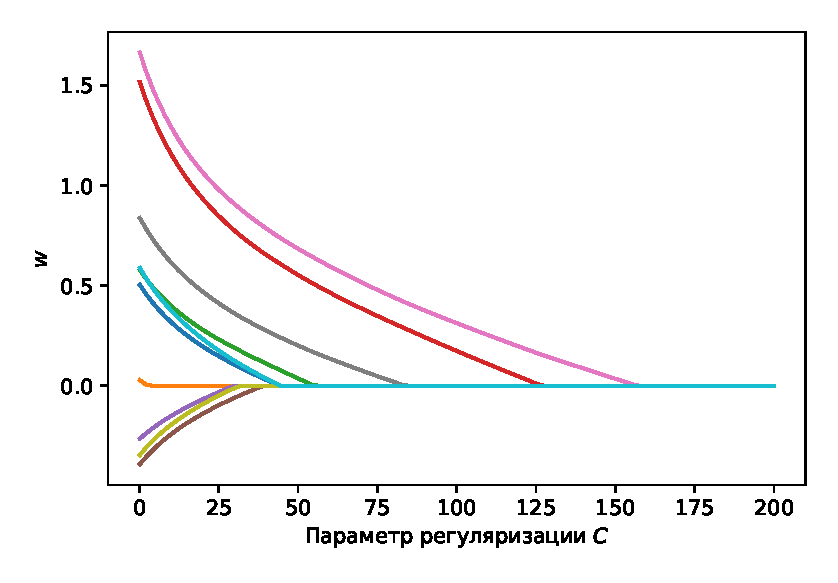
\includegraphics[width=0.5\textwidth]{../figures/log_reg_cs_exp.eps}
%	\caption{Sample figure caption.}
%	\label{fig:fig1}
%\end{figure}

\subsection{Tables}
%See awesome Table~\ref{tab:table}.

%The documentation for \verb+booktabs+ (`Publication quality tables in LaTeX') is available from:
%\begin{center}
%	\url{https://www.ctan.org/pkg/booktabs}
%\end{center}


%\begin{table}
%	\caption{Sample table title}
%	\centering
%	\begin{tabular}{lll}
%		\toprule
%		\multicolumn{2}{c}{Part}                   \\
%		\cmidrule(r){1-2}
%		Name     & Description     & Size ($\mu$m) \\
%		\midrule
%		Dendrite & Input terminal  & $\sim$100     \\
%		Axon     & Output terminal & $\sim$10      \\
%		Soma     & Cell body       & up to $10^6$  \\
%		\bottomrule
%	\end{tabular}
%	\label{tab:table}
%\end{table}

\subsection{Lists}
%\begin{itemize}
	%\item Lorem psum dolor sit amet
	%\item consectetur adipiscing elit.
	%\item Aliquam dignissim blandit est, in dictum tortor gravida eget. In ac %rutrum magna.
%\end{itemize}


\bibliographystyle{unsrtnat}
\bibliography{references}

\end{document}